% vim: set textwidth=120:

% Example CV based on the 1.5-column-cv template. Main features:
% * uses the Roboto font family and IcoMoon icon set;
% * doesn't use colours, different font weights are used instead for styling;
% * because the CV fits on one page, header and footer is empty, since there isn't much useful info to put there;
% * includes a photo.
\documentclass[a4paper]{article}


% package imports
% ---------------

\usepackage[english]{babel} % for correct language and hyphenation and stuff
\usepackage{calc}           % for easier length calculations (infix notation)
\usepackage{enumitem}       % for configuring list environments
\usepackage{fancyhdr}       % for setting header and footer
\usepackage{fontspec}       % for fonts
\usepackage{geometry}       % for setting margins (\newgeometry)
\usepackage{graphicx}       % for pictures
\usepackage{microtype}      % for microtypography stuff
\usepackage{xcolor}         % for colours
\usepackage{hyperref}       % for document links


\hypersetup {
    colorlinks=false,
}

% margin and column widths
% ------------------------

% margins
\newgeometry{left=10mm,right=10mm,top=10mm,bottom=10mm}

% width of the gap between left and right column
\newlength{\cvcolumngapwidth}
\setlength{\cvcolumngapwidth}{3.5mm}

% left column width
\newlength{\cvleftcolumnwidth}
\setlength{\cvleftcolumnwidth}{45mm}

% right column width
\newlength{\cvrightcolumnwidth}
\setlength{\cvrightcolumnwidth}{\textwidth-\cvleftcolumnwidth-\cvcolumngapwidth}

% set paragraph indentation to 0, because it screws up the whole layout otherwise
\setlength{\parindent}{0mm}


% style definitions
% -----------------
% style categories explanation:
% * \cvnameXXX is used for the name;
% * \cvsectionXXX is used for section names (left column, accompanied by a horizontal rule);
% * \cvtitleXXX is used for job/education titles (right column);
% * \cvdurationXXX is used for job/education durations (left column);
% * \cvheadingXXX is used for headings (left column);
% * \cvmainXXX (and \setmainfont) is used for main text;
% * \cvruleXXX is used for the horizontal rules denoting sections.

% font families
\defaultfontfeatures{Ligatures=TeX} % reportedly a good idea, see https://tex.stackexchange.com/a/37251

\newfontfamily{\cvnamefont}[Path=./Roboto/]{Roboto-Medium}
\newfontfamily{\cvsectionfont}[Path=./Roboto/]{Roboto-Light}
\newfontfamily{\cvtitlefont}[Path=./Roboto/]{Roboto-Regular}
\newfontfamily{\cvdurationfont}[Path=./Roboto/]{Roboto-LightItalic}
\newfontfamily{\cvheadingfont}[Path=./Roboto/]{Roboto-Regular}

\newfontfamily{\regularfont}[Path=./Roboto/]{Roboto-Regular}
\newfontfamily{\italicfont}[Path=./Roboto/]{Roboto-Italic}

\setmainfont[Path=./Roboto/]{Roboto-Light}


% colours
\definecolor{cvnamecolor}{HTML}{000000}
\definecolor{cvsectioncolor}{HTML}{000000}
\definecolor{cvtitlecolor}{HTML}{000000}
\definecolor{cvdurationcolor}{HTML}{000000}
\definecolor{cvheadingcolor}{HTML}{000000}
\definecolor{cvmaincolor}{HTML}{000000}
\definecolor{cvrulecolor}{HTML}{000000}

\color{cvmaincolor}

% styles
\newcommand{\cvnamestyle}[1]{{\Huge\cvnamefont\textcolor{cvnamecolor}{#1}}}
\newcommand{\cvsectionstyle}[1]{{\normalsize\cvsectionfont\textcolor{cvsectioncolor}{#1}}}
\newcommand{\cvtitlestyle}[1]{{\large\cvtitlefont\textcolor{cvtitlecolor}{#1}}}
\newcommand{\cvdurationstyle}[1]{{\small\cvdurationfont\textcolor{cvdurationcolor}{#1}}}
\newcommand{\cvheadingstyle}[1]{{\normalsize\cvheadingfont\textcolor{cvheadingcolor}{#1}}}

\newcommand{\italicstyle}[1]{{\small\italicfont\textcolor{cvsectioncolor}{#1}}}
\newcommand{\regularstyle}[1]{{\normalsize\regularfont\textcolor{cvsectioncolor}{#1}}}



% inter-item spacing
% ------------------

% vertical space after personal info and standard CV items
\newlength{\cvafteritemskipamount}
\setlength{\cvafteritemskipamount}{2mm plus 1.25mm minus 1.25mm}

% vertical space after sections
\newlength{\cvaftersectionskipamount}
\setlength{\cvaftersectionskipamount}{2mm plus 0.5mm minus 0.5mm}

% extra vertical space to be used when a section starts with an item with a heading (e.g. in the skills section),
% so that the heading does not follow the section name too closely
\newlength{\cvbetweensectionandheadingextraskipamount}
\setlength{\cvbetweensectionandheadingextraskipamount}{1mm plus 0.25mm minus 0.25mm}


% intra-item spacing
% ------------------

% vertical space after name
\newlength{\cvafternameskipamount}
\setlength{\cvafternameskipamount}{3mm plus 0.75mm minus 0.75mm}

% vertical space after personal info lines
\newlength{\cvafterpersonalinfolineskipamount}
\setlength{\cvafterpersonalinfolineskipamount}{1mm plus 0.5mm minus 0.5mm}

% vertical space after titles
\newlength{\cvaftertitleskipamount}
\setlength{\cvaftertitleskipamount}{1mm plus 0.25mm minus 0.25mm}

% value to be used as parskip in right column of CV items and itemsep in lists (same for both, for consistency)
\newlength{\cvparskip}
\setlength{\cvparskip}{0.5mm plus 0.125mm minus 0.125mm}

% set global list configuration (use parskip as itemsep, and no separation otherwise)
\setlist{parsep=0mm,topsep=0mm,partopsep=0mm,itemsep=\cvparskip}


% CV commands
% -----------

% creates a "personal info" CV item with the given left and right column contents, with appropriate vertical space after
% @param #1 left column content (should be the CV photo)
% @param #2 right column content (should be the name and personal info)
\newcommand{\cvpersonalinfo}[2]{
    % left and right column
    \begin{minipage}[t]{\cvleftcolumnwidth}
        \vspace{0mm} % XXX hack to align to top, see https://tex.stackexchange.com/a/11632
        \raggedleft #1
    \end{minipage}% XXX necessary comment to avoid unwanted space
    \hspace{\cvcolumngapwidth}% XXX necessary comment to avoid unwanted space
    \begin{minipage}[t]{\cvrightcolumnwidth}
        \vspace{0mm} % XXX hack to align to top, see https://tex.stackexchange.com/a/11632
        #2
    \end{minipage}

    % space after
    \vspace{\cvafteritemskipamount}
}

% typesets a name, with appropriate vertical space after
% @param #1 name text
\newcommand{\cvname}[1]{
    % name
    \cvnamestyle{#1}

    % space after
    \vspace{\cvafternameskipamount}
}

% typesets a line of personal info beginning with an icon, with appropriate vertical space after
% @param #1 parameters for the \includegraphics command used to include the icon
% @param #2 icon filename
% @param #3 line text
\newcommand{\cvpersonalinfolinewithicon}[3]{
    % icon, vertically aligned with text (see https://tex.stackexchange.com/a/129463)
    \raisebox{.5\fontcharht\font`E-.5\height}{\includegraphics[#1]{#2}}
    % text
    #3

    % space after
    \vspace{\cvafterpersonalinfolineskipamount}
}

% creates a "section" CV item with the given left column content, a horizontal rule in the right column, and with
% appropriate vertical space after
% @param #1 left column content (should be the section name)
\newcommand{\cvsection}[1]{
    % left and right column
    \begin{minipage}[t]{\cvleftcolumnwidth}
        \raggedleft\cvsectionstyle{#1}
    \end{minipage}% XXX necessary comment to avoid unwanted space
    \hspace{\cvcolumngapwidth}% XXX necessary comment to avoid unwanted space
    \begin{minipage}[t]{\cvrightcolumnwidth}
        \textcolor{cvrulecolor}{\rule{\cvrightcolumnwidth}{0.3mm}}
    \end{minipage}

    % space after
    \vspace{\cvaftersectionskipamount}
}

% creates a standard, multi-purpose CV item with the given left and right column contents, parskip set to cvparskip
% in the right column, and with appropriate vertical space after
% @param #1 left column content
% @param #2 right column content
\newcommand{\cvitem}[2]{
    % left and right column
    \begin{minipage}[t]{\cvleftcolumnwidth}
        \raggedleft #1
    \end{minipage}% XXX necessary comment to avoid unwanted space
    \hspace{\cvcolumngapwidth}% XXX necessary comment to avoid unwanted space
    \begin{minipage}[t]{\cvrightcolumnwidth}
        \setlength{\parskip}{\cvparskip} #2
    \end{minipage}

    % space after
    \vspace{\cvafteritemskipamount}
}

% typesets a title, with appropriate vertical space after
% @param #1 title text
\newcommand{\cvtitle}[1]{
    % title
    \cvtitlestyle{#1}

    % space after
    \vspace{\cvaftertitleskipamount}
    % XXX need to subtract cvparskip here, because it is automatically inserted after the title "paragraph"
    \vspace{-\cvparskip}
}


% header and footer
% -----------------

% set empty header and footer
\pagestyle{empty}



% preamble end/document start
% ===========================

\begin{document}


% personal info
% -------------

\cvpersonalinfo{
    % photo
    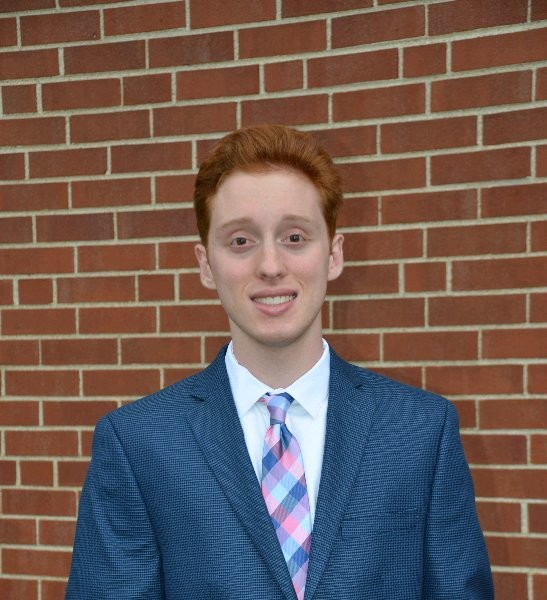
\includegraphics[height=40mm]{img/me.png}
}{
    % name
    \cvname{Chris Cohen}

    % address
    \cvpersonalinfolinewithicon{height=4mm}{img/location.png}{
        20 Littleton Street, Apt. 12, West Lafayette, IN 47906
    }

    % phone number
    \cvpersonalinfolinewithicon{height=4mm, width=4mm}{img/phone.png}{
      (636)\ 675-9358
    }

    % email address
    \cvpersonalinfolinewithicon{height=4mm}{img/email.png}{
      chriscohen@chriscohen.dev
    }

    % LinkedIn account
    \cvpersonalinfolinewithicon{height=4mm}{img/linkedin.png}{
      \href{https://www.linkedin.com/in/chris-cohen-purdue/}{https://www.linkedin.com/in/chris-cohen-purdue/}
    }

    % Website
    \cvpersonalinfolinewithicon{height=4mm}{img/website.png}{
      \href{https://www.chriscohen.dev}{https://www.chriscohen.dev}
    }

    % GitHub
    \cvpersonalinfolinewithicon{height=4mm}{img/github.png}{
      \href{https://github.com/cohenchris}{https://github.com/cohenchris}
    }
}

% education
% ---------

\cvsection{\LARGE EDUCATION}

% bachelor's
\cvitem{
    \cvdurationstyle{Aug. 2017 -- Present}
}{
    \cvtitle{Bachelor of Science (Software Engineering and Cybersecurity)}

    \italicstyle{Purdue University}

    \begin{itemize}[leftmargin=*]
        \item 3.83 GPA
        \item 6x Dean's List, 5x Semester Honors
    \end{itemize}
}

% work experience
% ---------------

\cvsection{\LARGE EMPLOYMENT}

% Qualcomm
\cvitem{
    \cvdurationstyle{May 2020 -- Present}
}{
    \cvtitle{Qualcomm, QGOV Division}

    \italicstyle{Embedded Software Engineering Intern}

    \normalsize
    \begin{itemize}[leftmargin=*]
        \item TBD
    \end{itemize}
    \vspace{2mm}
}

% NSWC Crane
\cvitem{
    \cvdurationstyle{May 2019 -- Aug. 2019}
}{

    \cvtitle{Naval Surface Warface Center, Crane Division}

    \italicstyle{Software Engineering Intern}

    \normalsize
    \begin{itemize}[leftmargin=*]
        \item Improved US Navy missile sustainment efforts by upgrading an existing
natural language processing algorithm to process failure databases.
        \item Held a valid ‘secret’ level security clearance given by the US Government.
    \end{itemize}
}

% skills
% ------

\cvsection{\LARGE EXPERTISE}

% programming languages
\cvitem{
    \cvheadingstyle{Languages}
}{
  C \hspace{12mm} C++ \hspace{12mm} Python \hspace{12mm} ARM/x86 Assembly \hspace{12mm} Bash \hspace{12mm} Javascript
  \vspace{2mm}
}

% topics
\cvitem{
    \cvheadingstyle{Memory Management}
}{
    \begin{itemize}[leftmargin=*]
      \item Paging, Virtualization
      \item Cache Memory Hierarchy
      \item Stack and Heap Management for ARM/x86
    \end{itemize}
  \vspace{3mm}
}

\cvitem{
    \cvheadingstyle{OS and Systems Programming}
}{
    \begin{itemize}[leftmargin=*]
      \item Software/Hardware Interrupts and Device Management
      \item Asynchronous Inter-Process Communication
      \item Return-Oriented Programming
      \item Concurrency and Parallelism (Semaphores, Locks, Forking, Threading, Scheduling)
    \end{itemize}
  \vspace{3mm}
}

\cvitem{
    \cvheadingstyle{OSI/ISO 7-Layer Model}
}{
    \begin{itemize}[leftmargin=*]
      \item TCP, UDP, HTTP
      \item IP addressing/routing, DHCP, DNS translation
      \item MAC addressing/routing, ARP
      \item Basic cryptography and security approaches
    \end{itemize}
}

% education
% ---------

\cvsection{\LARGE PROJECTS}

% Honeypot
\cvitem{
    \cvdurationstyle{April 2020}
}{
  \cvtitle{Web Server Honeypot (Extracurricular)}

    \begin{itemize}[leftmargin=*]
        \item Hosted an HTTPS Honeypot Server to lure attackers and collect information
        \item Graphical directory browsing and support for 14 HTTP response codes
        \item Automatic blacklisting for clients who send too many requests too quickly
        \item Analyzed logs and learned about different types of attacks on web servers
    \end{itemize}
    \vspace{2mm}
}

% 
\cvitem{
    \cvdurationstyle{March 2020}
}{
  \cvtitle{Process Hijacking in XINU (Operating Systems)}

    \begin{itemize}[leftmargin=*]
        \item Manipulated a victim process by locating and modifying return addresses and local variables in the runtime stack
        \item Learned about protection against this sort of attack (i.e. stack canaries)
        \item Studied how x86 interrupts, system calls, and function calls affect the runtime stack
    \end{itemize}
    \vspace{2mm}
}

\cvitem{
    \cvdurationstyle{Sept. 2019 -- Oct. 2019}
}{
  \cvtitle{Shell Interpreter in C (Systems Programming)}

    \begin{itemize}[leftmargin=*]
        \item Parsing and execution of commands
        \item File redirection and piping
        \item Signal handling and inter-process communication
        \item Subshell execution via forking
    \end{itemize}
}

\end{document}
